\documentclass[12pt]{amsart}
\usepackage[letterpaper, portrait, left = 1in, right = 1in, top = 1.2in, bottom=1.5in]{geometry} 
%\usepackage{setspace} \doublespacing
%\usepackage[letterpaper, portrait, margin=1.3in]{geometry}
\usepackage[table,xcdraw]{xcolor}
\usepackage{amssymb}
\usepackage{amsfonts}
\usepackage{longtable}
\usepackage{amsmath,amsthm}
\usepackage{enumitem}
\usepackage[utf8]{inputenc}
\usepackage{mathtools}
\usepackage{graphicx}
\usepackage{parskip}
\usepackage{multicol}
\usepackage{listings}
\usepackage[skip=0.25pt]{caption}
\usepackage[mathscr]{euscript}
\usepackage{quiver}
\setlength{\parindent}{0pt}
\usepackage{thm-restate}
\definecolor{vividburgundy}{rgb}{0.62, 0.11, 0.21}
\usepackage[driverfallback=hypertex,pagebackref=false,colorlinks,citecolor=vividburgundy]{hyperref}
\usepackage[capitalize]{cleveref}
%\usepackage[cmintegrals,cmbraces]{newtxmath}
%\usepackage{ebgaramond-maths}

%\usepackage{fourier}
%----------FONT OPTIONS----------
% sans-serif
%\usepackage[sfdefault]{FiraSans}
 %\usepackage[sfdefault]{roboto}
% \usepackage[sfdefault]{noto-sans}
%\usepackage[default]{sourcesanspro}

% serif
%\usepackage{CormorantGaramond}

%\usepackage{charter}
\usepackage[T1]{fontenc}
\usepackage{cleveref}
\definecolor{dg}{RGB}{10, 100, 10}
\setlength{\parindent}{0in}
\renewcommand{\qed}{$\hfill\blacksquare$}
% \newtheoremstyle{style}{2pt}{1pt}{\normalfont}{}{\bfseries}{\\}{0cm}{}
% \theoremstyle{style}
\newtheorem{lemma}{Lemma}[section]
% \newtheorem{lemma}{Lemma}
\newtheorem{thm}[lemma]{Theorem}
\newtheorem{prop}[lemma]{Proposition}
\newtheorem{cor}[lemma]{Corollary}
\newtheorem{conj}[lemma]{Conjecture}
\newtheorem{cl}[lemma]{Claim}
\newtheorem{rmk}{Remark}
\newtheorem{defn}[lemma]{Definition}
\newtheorem{qs}{Question}
\newtheoremstyle{styleS}{}{}{\color{dg}}{}{\color{dg}\bfseries}{. }{0cm}{}
\theoremstyle{styleS}
\newtheorem*{sol}{Solution}
\newtheoremstyle{style1}{}{}{\normalfont}{}{\bfseries}{. }{0cm}{}
\theoremstyle{style1}
\newtheorem{prob}{Problem}[section]
\newtheorem*{prb}{Problem}
\newtheoremstyle{style2}{1pt}{4pt}{\normalfont}{}{\itshape}{. }{0cm}{}
\theoremstyle{style2}
\newtheorem{ex}[lemma]{Example}
\newtheorem*{pf}{Proof}

\newcommand{\norm}[2]{
\left\lVert #1 \right\rVert_{#2}
}
\usepackage{mathrsfs}
%\usepackage[table,xcdraw]{xcolor}
\usepackage{booktabs}
\usepackage{tikz}
\usetikzlibrary{matrix}
\renewcommand{\l}{\ell}


\newcommand{\fA}{{\mathfrak{A}}}   \newcommand{\fB}{{\mathfrak{B}}}
\newcommand{\fC}{{\mathfrak{C}}}   \newcommand{\fD}{{\mathfrak{D}}}
\newcommand{\fE}{{\mathfrak{E}}}   \newcommand{\fF}{{\mathfrak{F}}}
\newcommand{\fG}{{\mathfrak{G}}}   \newcommand{\fH}{{\mathfrak{H}}}
\newcommand{\fI}{{\mathfrak{I}}}   \newcommand{\fJ}{{\mathfrak{J}}}
\newcommand{\fK}{{\mathfrak{K}}}   \newcommand{\fL}{{\mathfrak{L}}}
\newcommand{\fM}{{\mathfrak{M}}}   \newcommand{\fN}{{\mathfrak{N}}}
\newcommand{\fO}{{\mathfrak{O}}}   \newcommand{\fP}{{\mathfrak{P}}}
\newcommand{\fQ}{{\mathfrak{Q}}}   \newcommand{\fR}{{\mathfrak{R}}}
\newcommand{\fS}{{\mathfrak{S}}}   \newcommand{\fT}{{\mathfrak{T}}}
\newcommand{\fU}{{\mathfrak{U}}}   \newcommand{\fV}{{\mathfrak{V}}}
\newcommand{\fW}{{\mathfrak{W}}}   \newcommand{\fX}{{\mathfrak{X}}}
\newcommand{\fY}{{\mathfrak{Y}}}   \newcommand{\fZ}{{\mathfrak{Z}}}

\newcommand{\cA}{{\mathcal{A}}}   \newcommand{\cB}{{\mathcal{B}}}
\newcommand{\cC}{{\mathcal{C}}}   \newcommand{\cD}{{\mathcal{D}}}
\newcommand{\cE}{{\mathcal{E}}}   \newcommand{\cF}{{\mathcal{F}}}
\newcommand{\cG}{{\mathcal{G}}}   \newcommand{\cH}{{\mathcal{H}}}
\newcommand{\cI}{{\mathcal{I}}}   \newcommand{\cJ}{{\mathcal{J}}}
\newcommand{\cK}{{\mathcal{K}}}   \newcommand{\cL}{{\mathcal{L}}}
\newcommand{\cM}{{\mathcal{M}}}   \newcommand{\cN}{{\mathcal{N}}}
\newcommand{\cO}{{\mathcal{O}}}   \newcommand{\cP}{{\mathcal{P}}}
\newcommand{\cQ}{{\mathcal{Q}}}   \newcommand{\cR}{{\mathcal{R}}}
\newcommand{\cS}{{\mathcal{S}}}   \newcommand{\cT}{{\mathcal{T}}}
\newcommand{\cU}{{\mathcal{U}}}   \newcommand{\cV}{{\mathcal{V}}}
\newcommand{\cW}{{\mathcal{W}}}   \newcommand{\cX}{{\mathcal{X}}}
\newcommand{\cY}{{\mathcal{Y}}}   \newcommand{\cZ}{{\mathcal{Z}}}

\newcommand{\sA}{{\mathscr{A}}}   \newcommand{\sB}{{\mathscr{B}}}
\newcommand{\sC}{{\mathscr{C}}}   \newcommand{\sD}{{\mathscr{D}}}
\newcommand{\sE}{{\mathscr{E}}}   \newcommand{\sF}{{\mathscr{F}}}
\newcommand{\sG}{{\mathscr{G}}}   \newcommand{\sH}{{\mathscr{H}}}
\newcommand{\sI}{{\mathscr{I}}}   \newcommand{\sJ}{{\mathscr{J}}}
\newcommand{\sK}{{\mathscr{K}}}   \newcommand{\sL}{{\mathscr{L}}}
\newcommand{\sM}{{\mathscr{M}}}   \newcommand{\sN}{{\mathscr{N}}}
\newcommand{\sO}{{\mathscr{O}}}   \newcommand{\sP}{{\mathscr{P}}}
\newcommand{\sQ}{{\mathscr{Q}}}   \newcommand{\sR}{{\mathscr{R}}}
\newcommand{\sS}{{\mathscr{S}}}   \newcommand{\sT}{{\mathscr{T}}}
\newcommand{\sU}{{\mathscr{U}}}   \newcommand{\sV}{{\mathscr{V}}}
\newcommand{\sW}{{\mathscr{W}}}   \newcommand{\sX}{{\mathscr{X}}}
\newcommand{\sY}{{\mathscr{Y}}}   \newcommand{\sZ}{{\mathscr{Z}}}

\newcommand{\ta}{{\tilde{a}}}   \newcommand{\tb}{{\tilde{b}}}
\newcommand{\tc}{{\tilde{c}}}   \newcommand{\td}{{\tilde{d}}}
\newcommand{\te}{{\tilde{e}}}   \newcommand{\tf}{{\tilde{f}}}
\newcommand{\tg}{{\tilde{g}}}   
\newcommand{\ti}{{\tilde{i}}}   \newcommand{\tj}{{\tilde{j}}}
\newcommand{\tk}{{\tilde{k}}}   \newcommand{\tl}{{\tilde{l}}}
\newcommand{\tm}{{\tilde{m}}}   \newcommand{\tn}{{\tilde{n}}}
		         	\newcommand{\tp}{{\tilde{p}}}
\newcommand{\tq}{{\tilde{q}}}   \newcommand{\tr}{{\tilde{r}}}
\newcommand{\ts}{{\tilde{s}}}   
\newcommand{\tu}{{\tilde{u}}}   \newcommand{\tv}{{\tilde{v}}}
\newcommand{\tw}{{\tilde{w}}}   \newcommand{\tx}{{\tilde{x}}}
\newcommand{\ty}{{\tilde{y}}}   \newcommand{\tz}{{\tilde{z}}}

\newcommand{\red}{{\color{red}red}}
\newcommand{\blue}{{\color{blue}blue}}

\newcommand{\into}{\hookrightarrow}
\newcommand{\onto}{\twoheadrightarrow}
\newcommand\N{\ensuremath{\mathbb{N}}}

%\newcommand\L{\ensuremath{\mathbb{L}}}
\newcommand{\bP}{\mathbb{P}}
\newcommand\M{\ensuremath{\mathbb{M}}}
\newcommand\R{\ensuremath{\mathbb{R}}}
\newcommand\Z{\ensuremath{\mathbb{Z}}}
\renewcommand\O{\ensuremath{\emptyset}}
\newcommand\Q{\ensuremath{\mathbb{Q}}}
\newcommand\C{\ensuremath{\mathbb{C}}}
\newcommand{\K}{\ensuremath{\mathbb{K}}}
\newcommand\F{\ensuremath{\mathbb{F}}}
\newcommand{\aff}{\ensuremath{\mathbb{A}}}
\newcommand{\proj}{\ensuremath{\mathbb{P}}}
\newcommand{\dd}{\mathrm{d}}
\newcommand{\m}{\ensuremath{\mathfrak{m}}}
\newcommand{\p}{\ensuremath{\mathfrak{p}}}
\newcommand{\n}{\ensuremath{\mathfrak{n}}}
\renewcommand{\phi}{\varphi}
\renewcommand{\qedsymbol}{\ensuremath{\blacksquare}}
%\newcommand{\st}{\;|\;}
\newcommand{\st}{%
  \nonscript\;
  \ifnum\currentgrouptype=16
    \;\middle|\;
  \else
    \;|\;
  \fi
  \nonscript\;}
\newcommand{\ltr}{\par \noindent \framebox[1\width]{ $\implies$ } \hspace{.2cm}}
\newcommand{\rtl}{\par \noindent \framebox[1\width]{ $\impliedby$ } \hspace{.2cm} }
\newcommand{\abs}[1]{\left| #1 \right|}
\newcommand{\inner}[2]{\left\langle #1, #2 \right\rangle}
\newcommand{\E}[1]{\mathbb E\left[ #1 \right]}
\newcommand{\e}[1]{\exp\left( #1 \right)}
\renewcommand{\P}[1]{\mathbb P\left[ #1 \right]}
\newcommand{\Var}[1]{\text{Var}\left[ #1 \right]}
\newcommand*\circled[1]{\tikz[baseline=(char.base)]{
            \node[shape=circle,draw,inner sep=2pt] (char) {#1};}}
\newcommand{\ds}{\displaystyle}

\DeclareMathOperator{\sym}{Sym}
\DeclareMathOperator{\mds}{MDS}
\DeclareMathOperator{\Tor}{Tor}
\DeclareMathOperator{\Ext}{Ext}
\DeclareMathOperator{\adj}{adj}
\DeclareMathOperator{\Tr}{Tr}
\DeclareMathOperator{\GL}{GL}
%\DeclareMathOperator{\Tr}{Tr}
\DeclareMathOperator{\orbit}{Or}
\DeclareMathOperator{\stab}{Stab}
\DeclareMathOperator{\fix}{Fix}
\DeclareMathOperator{\re}{Re}
\DeclareMathOperator{\im}{Im}
\DeclareMathOperator{\ord}{Ord}
\DeclareMathOperator{\mspec}{mSpec}
\DeclareMathOperator{\spec}{Spec}
\DeclareMathOperator{\frob}{Frob}
\DeclareMathOperator{\id}{Id}
\DeclareMathOperator{\colim}{colim}
\DeclareMathOperator{\loc}{loc}
\DeclareMathOperator{\res}{Res}
\DeclareMathOperator{\rad}{rad}
\DeclareMathOperator{\Res}{Res}
\DeclareMathOperator{\diam}{diam}
\DeclareMathOperator{\arcsec}{arcsec}
\DeclareMathOperator{\arccot}{arccot}
\DeclareMathOperator{\len}{len}
\DeclareMathOperator{\area}{area}
\DeclareMathOperator{\vol}{vol}
\DeclareMathOperator{\ev}{ev}
\DeclareMathOperator{\sgn}{sgn}
\DeclareMathOperator{\supp}{supp}
\DeclareMathOperator{\diff}{d}
\DeclareMathOperator{\Dom}{Dom}
\DeclareMathOperator{\rk}{rank}
\renewcommand{\d}{\diff}
\let\oldend\endlinechar
\renewcommand{\endlinechar}{\oldend}
\newcommand{\open}{\underset{\text{open}}{\subset}}
\newcommand{\divides}{\mathbin{|}}
\newcommand{\set}[1]{\ensuremath{\left\{#1\right\}}}
\newcommand{\sett}{\coloneqq}
\newcommand*\isomap{%
  \xrightarrow{\raisebox{-0.9ex}[0ex][0ex]{$\sim$}}%
}
\renewcommand{\epsilon}{\varepsilon}
\newcommand{\fa}{~\forall~}
%\usepackage[nobottomtitles*]{titlesec}
\usepackage{titletoc}
%\titleformat{\section}[runin]
%{\normalfont\Large\bfseries}
%{}{0pt}{}%
%[\ifthenelse{\equal{\thesection}{0}}{\\\vspace*{0pt}}{\space\thesection}]
\newcommand{\sint}{\sin\theta}
\newcommand{\cost}{\cos\theta}
\newcommand{\tant}{\tan\theta}
\newcommand{\lb}{\left[}
\newcommand{\rb}{\right]}
\newcommand{\lp}{\left(}
\newcommand{\rp}{\right)}
\newcommand{\br}[1]{\lb#1\rb}
\newcommand{\pa}[1]{\lp#1\rp}
\usepackage{pdfpages}
\usepackage{fancyhdr}
	\pagestyle{fancyplain}
	\fancyhf{}
	\fancyhead[C]{\thepage}

\usepackage{wrapfig}
\usepackage{multicol}
\usepackage[breakable]{tcolorbox}
\usepackage{algorithm}
\usepackage{algpseudocode}
\usepackage[framed,numbered,autolinebreaks,useliterate]{mcode}
\usepackage{float}
%\usepackage{listings}
%\fontfamily{qcr}\selectfont 
%\usepackage[backend=bibtex]{biblatex}
\usepackage[
backend=biber,
style=alphabetic,%firstinits,
citestyle=ieee-alphabetic,
%natbib=true,
%uniquelist=false,
maxnames=10,
sorting=ynt
]{biblatex}
%\addbibresource{writeup/article/refs.bib}
%\title{\vspace{-1cm}}
\title{\textbf{CONVEX AND CONIC OPTIMIZATION}\\ Endterm}
\usepackage{quiver}
\usepackage[nobottomtitles*]{titlesec}
\usepackage{titletoc}
\titleformat{\section}[runin]
  {\normalfont\Large\bfseries}
  {}{0pt}{}%
  [\ifthenelse{\equal{\thesection}{0}}{\\\vspace*{0pt}}{\space\thesection}]
\author{{\Large NILAVA METYA} \\ 
\href{mailto:nilava.metya@rutgers.edu}{nilava.metya@rutgers.edu}\\
\href{mailto:nm8188@princeton.edu}{nm8188@princeton.edu}}
\date{May $12$, $2024$}
\newcommand{\pb}{\section{Problem}~\par}
\newcommand{\soln}{\subsection*{Solution}}
\newcommand{\conv}{\text{conv}}
\newcommand{\epi}{\text{epi}}
\usepackage{pdfpages}
\usepackage{fancyhdr}
	\pagestyle{fancyplain}
	\fancyhf{}
	\fancyhead[R]{\thepage}
\setlength{\columnsep}{1.2cm}
\newcommand{\fa}{~\forall}
\begin{document}

\maketitle

\pb
Suppose a set $S \subseteq \R^{n}$ is nonempty, convex, and closed and that its complement $\overline S$, i.e., the set $\R^{n}\smallsetminus S$, is convex and nonempty. Show that $S$ must be a halfspace.

\soln

Since $S,\overline S$ are both convex, $\exists a\in \R^{n}\smallsetminus\set{0}, b\in\R$ such that $a^{\top}x\le b~\forall x\in S$ and $a^{\top}x \ge b~\forall x\in \overline S$ (we could use separating hyperplane theorem because $S,\overline S$ are non-empty convex sets that don't intersect). Let $T = \set{x\in\R^{n}\st a^{\top}x \le b}$. The above shows that $S\subseteq T$. We want to show $T\subseteq S$, in other words, $\overline S \subseteq \overline T = \set{x\in\R^{n}\st a^{\top}x >b}$. 

We are done if we show that $x\in \overline S\implies a^{\top}x \ne b$. For the sake of contradiction, suppose $x\in \overline S$ is such that $a^{\top}x = b$. $\overline S$ is open (because $S$ is closed), so $\exists r>0$ such that $B^{o}_{2r}(x)\sett \set{y\in\R^{n}\st \norm{y-x}{2} < 2r}\subseteq \overline S$. Consider the vector $y \sett x-\frac{r}{\norm{a}{}}a$. Then $\norm{y-x}{} = r$ whence $y\in B^{o}_{2r}(x)\subseteq \overline S$. However $a^{\top}y = a^{\top}\left(x-\frac{r}{\norm{a}{}}a\right) = b - r \norm{a}{} < b$. But we saw earlier that inner product of $a$ with any point in $\overline S$ must be at least $b$. This is a contradiction. It follows that $a^{\top}x< b~\forall x\in\overline S$. And thus $S = T = \set{x\in\R^{n}\st a^{\top}x\le b}$ which is a halfspace.



\newpage




\pb
For a graph $G$ on $n$ vertices, let $\alpha(G)$ be the stability number of $G$, $\vartheta(G)$ be the Lov\'asz theta number of $G$, and $\vartheta'(G)$ be the optimal value of the semidefinite program:
\begin{equation}\label{lovasz}\tag{$(Q)$}
\vartheta'(G) = \left\{
\begin{aligned}
\min_{\substack{P\in S^{n}\\k\in \R}}&~ k\\
\text{s.t.} &~ k(I+A)-J-P \ge 0\\
&~ P\succeq 0
\end{aligned}\right.
\end{equation}
\begin{enumerate}[leftmargin=*, label=(\alph*)]
\item Show that $\alpha(G)\le \vartheta'(G)\le \vartheta(G)$
\item Let $G$ be the graph with vertex set corresponding to all the vectors in $\set{0,1}^{6}$, two distinct vectors being adjacent if their $\ell_{1}$ distance (i.e., Hamming distance) is less than $4$. For your convenience, the adjacency matrix of this graph is given in the file \texttt{AdjacencyMatrix.mat}. Compute $\alpha(G),\vartheta'(G)$, and $\vartheta(G)$.
\end{enumerate}

\soln

\begin{enumerate}[leftmargin=*, label=(\alph*)]
\item \underline{Proof of $\alpha(G)\le \vartheta'(G)$}: Say $(P,k)$ is feasible to \ref{lovasz}. Consider an arbitrary $x\in \R^{n}$ and $x\ge 0$. Then $k x^{\top}(I+A)x - x^{\top}Jx \ge x^{\top} Px$ because of the first constraint. Using the positive semi-definiteness of $P$ we get $k x^{\top}(I+A)x \ge x^{\top}Jx$. However $\ds x^{\top}Jx = \left(\sum_{i=1}^{n}x_{i}\right)^{2}$. Furthermore, if $x\in \Delta_{n-1} = \set{p\in \R^{n} : p\ge 0, \norm{p}{1} = 1}$, then the above satisfy that $x^{\top}(I+A)x \ge \frac{1}{k}$. \\
Recall that the Motzkin-Strauss theorem says that $\ds\frac{1}{\alpha(G)}=\min_{x\in \Delta_{n-1}} x^{\top}(A+I)x$. But we have $x^{\top}(I+A)x \ge \frac{1}{k}~\forall x\in \Delta_{n-1}$. Thus $\alpha(G)\le k$. Here $k$ is itself the objective value of any feasible point in the optimization problem \ref{lovasz}. Since $\alpha(G)$ is a lower bound of the objective of any feasible point in \ref{lovasz}, it must also be a lower bound of the optimal value $\vartheta'(G)$.

\underline{Proof of $\vartheta'(G)\le\vartheta(G)$}:
{\color{gray}\textbf{Discussion}: The inequations in \ref{lovasz} hint at the dual of the Lovasz SDP: $\min\set{t:(t,Z)\in \R\times S^{n}, Z_{ij}=0\forall \set{i,j}\notin E, tI+Z\succeq J}$. This is from equation $(7)$ in Lecture 11. The expectation is that after transforming the PSD constraints in \ref{lovasz}, it will look similar to the PSD constraints of the Lovasz SDP, and the other constraints in \ref{lovasz} will be a relaxation. The first instinct was to take $kI+Z-J = P$ so that $k(I+A)-J-P = kA-Z$. As an attempt, I also tried taking the dual of this program and it seemed to be close to the original Lovasz SDP but I did not know how to prove that there is no duality gap. So it made sense to start with the dual of the SDP.}

Consider \ref{lovasz} along with the following three optimization problems
\begin{multicols}{3}
\begin{equation}\label{tra}\tag{$(R)$}
\begin{aligned}
\min_{\substack{X\in S^{n}\\k\in \R}}&~ k\\
\text{s.t.} &~ kA \ge X\\
&~ kI+X\succeq J
\end{aligned}
\end{equation}
\begin{equation}\label{rel}\tag{$(S)$}
\begin{aligned}
\min_{\substack{X\in S^{n}\\k\in\R}}&~ k\\
\text{s.t.} &~ X_{ij} \le 0 ~\forall \set{i,j}\in \overline E\\
&~X_{ii} \le 0 ~\forall i\in[n]\\
&~ kI+X\succeq J
\end{aligned}
\end{equation}
\begin{equation}\label{theta}\tag{$(L)$}
\begin{aligned}
\min_{\substack{Z\in S^{n}\\k\in\R}}&~ k\\
\text{s.t.} &~ Z_{ij} = 0 ~\forall \set{i,j}\in \overline E\\
&~Z_{ii} = 0 ~\forall i\in[n]\\
&~ kI+Z\succeq J
\end{aligned}
\end{equation}
\end{multicols}

\begin{cl}
\text{optval}\ref{lovasz} $=$ \text{optval}\ref{tra}.
\end{cl}
\begin{proof}
Take $X = P+J-kI$ to get \ref{tra} from \ref{lovasz} (and take $P=kI+X-J$ for the other way). $k(I+A)-J-P\ge 0\iff kA\ge X$. $P\succeq 0\iff kI+X\succeq J$. Objectives are same.
\end{proof}


\begin{cl}
\text{optval}\ref{tra} $\le$ \text{optval}\ref{rel}.
\end{cl}
\begin{proof}
{\color{gray}(These values are in fact equal, but we'll only prove the given inequality.)}\\
Say $(X,k)$ is feasible to \ref{rel}. So $X_{ij}\le 0~\forall \set{i,j}\notin E$ ($\set{i,j}\notin E$ is satisfied for the case $i=j$) and $kI+X-J\succeq 0$. Let's show that $(X,k)$ is feasible to \ref{tra}. The PSD criteria are the same, so we need not worry about that.\\
Pick an edge $\set{i,j}\in E$. Then 
\begin{align*}
0&\le (e_{i}-e_{j})^{\top}(kI+X-J)(e_{i}-e_{j}) \\
&= (kI_{ii}+X_{ii}-J_{ii}) + (kI_{jj}+X_{jj}-J_{jj}) - 2(kI_{ij}+X_{ij}-J_{ij})\\
&= (k+X_{ii}-1)+(k+X_{jj}-1) - 2(X_{ij}-1)\\
\implies 2(X_{ij}-1)&\le 2(k-1) + X_{ii} + X_{jj} \le 2(k-1)\\
\implies X_{ij} &\le k
\end{align*}

Thus if $\set{i,j}\in E$ then $X_{ij}\le k = k\cdot A_{ij}$ as shown above.\footnote{Another direct way to argue is that the maximum absolute value of a PSD matrix occurs on diagonal and the diagonal has non-negative entries so $k-1\ge k+X_{ii}-1 = \abs{k+X_{ii}-1} \ge \abs{0+X_{ij}-1} \ge X_{ij}-1$.} If $\set{i,j}\notin E$ then $X_{ij}\le 0 = k\cdot A_{ij}$ anyway. So $X\le kA$.
\end{proof}

\begin{cl}
\text{optval}\ref{rel} $\le$ \text{optval}\ref{theta}.
\end{cl}
\begin{proof}
The constraints are simply relaxed from ``$=0$'' in \ref{theta} to ``$\le 0$'' in \ref{rel}. So the feasible set of \ref{rel} contains that of \ref{theta}. Minimizing over a larger set (i.e., in \ref{rel}) gives (non-strict) smaller values. So the given claim holds.
\end{proof}

Combining the above claims gives $\vartheta'(G) = $ optval\ref{lovasz} $\le$ optval\ref{theta} $=\vartheta(G)$.


\item See code next page. 

The Lovasz SDP gives $\vartheta(G) = 5.\overline{3}$ (rounding to the nearest sensible/intuitive number).

In order to find $\alpha(G)$, we start by checking whether there is a stable set of size $5$ (as indicated by Lovasz SDP). That fails. So we check for a stable set of size $4$ and we find many. One of them is given by vertices $0,15,51,60$ (indexing at $0$). This has been checked in the code: the submatrix corresponding to these rows and columns is all $0$. So $\alpha(G) = 4$ because there is no stable set of size $5$, but there are stable sets of size $4$. 


But the given optimization problem has optimal value $\vartheta'(G)=4$ (since it's $3.99999\cdots$ and we proved that it's an upper bound on $\alpha(G)$ and taking the closest sensible answer keeping in mind numerical errors). 

Thus the given optimization solution is tight, while the Lovasz SDP has a gap.

{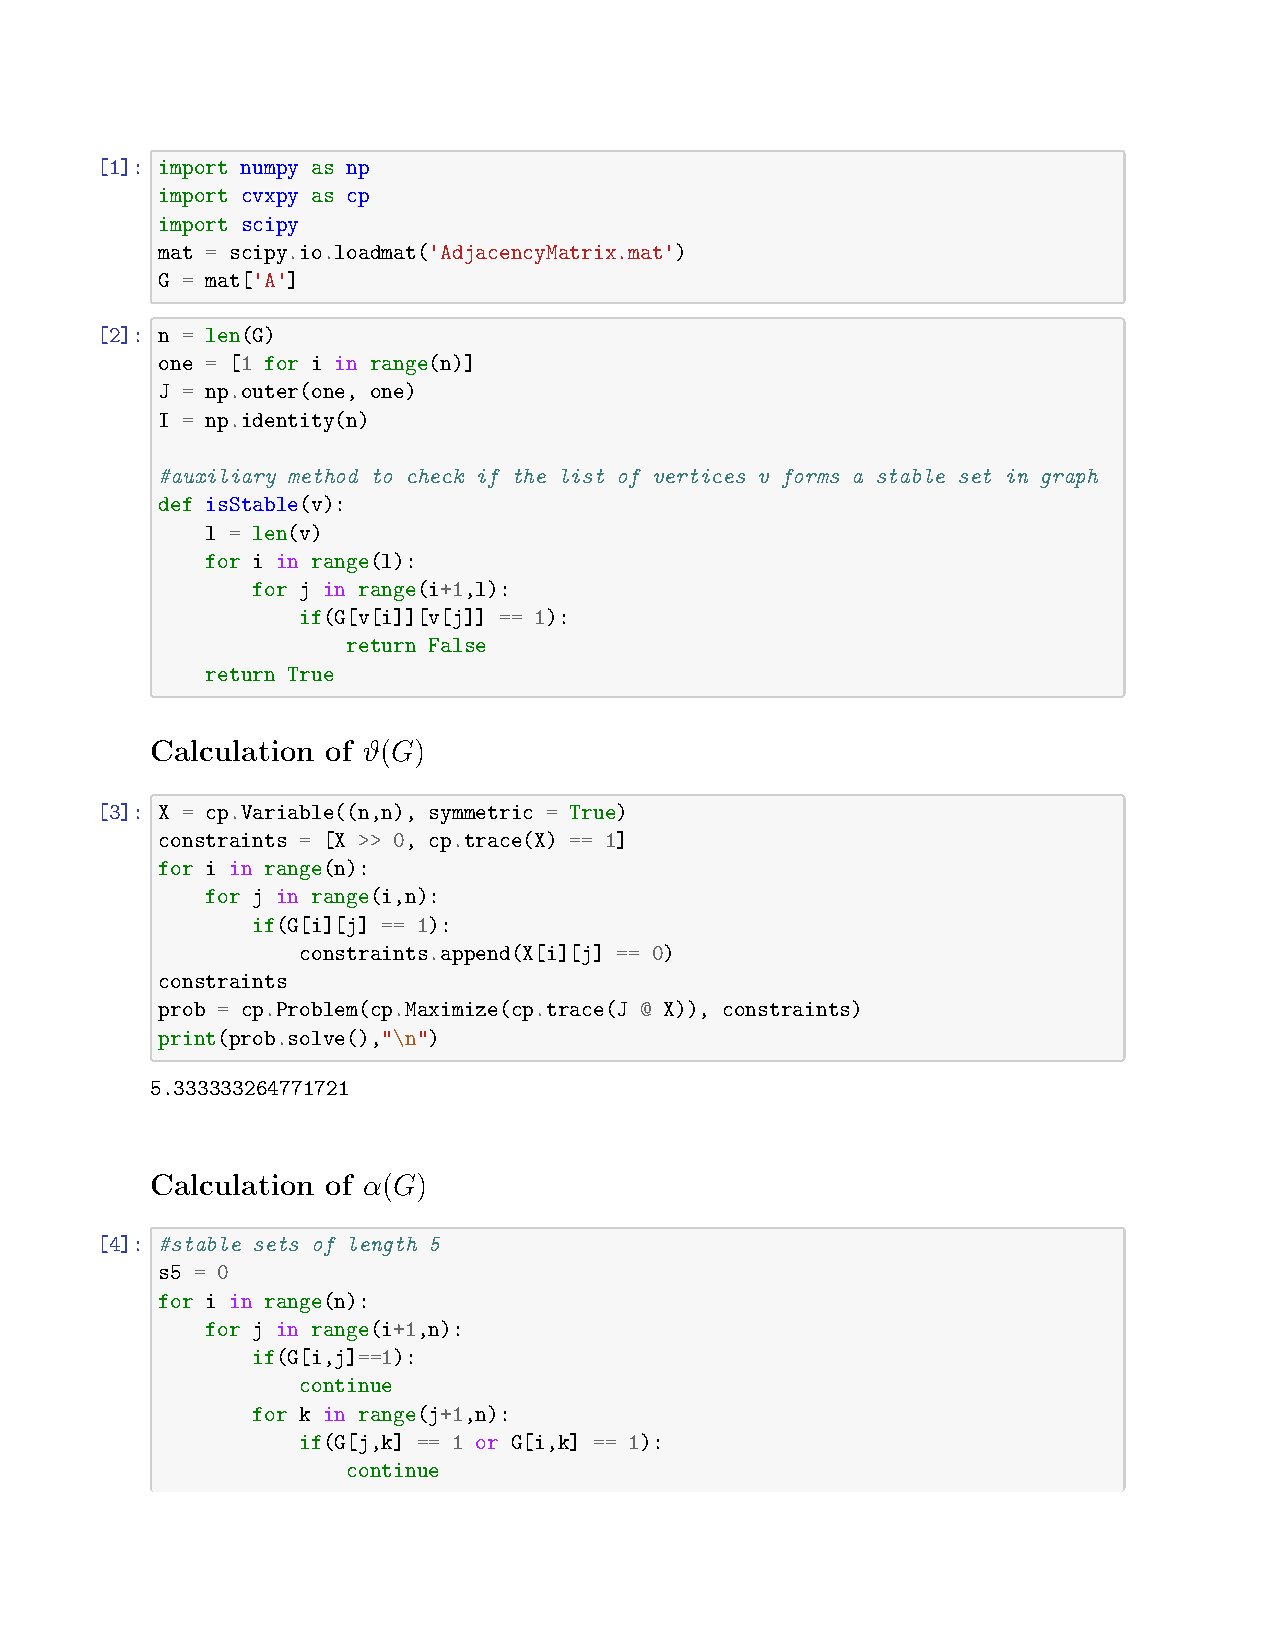
\includepdf[pages=-,pagecommand={\label{pdf:code}}]{Graph/Graph_alphatheta.pdf}}




\end{enumerate}



\newpage
\pb

Show that the following decision problem is NP-complete. \textbf{CONCAVE-BOX-QP}: Given a symmetric matrix $Q\in \Q^{n\times n}$, with $Q\preceq 0$, vectors $c,l,u\in \Q^{n}$, and a scalar $k \in \Q$, decide whether the optimal value of the following optimization problem is less than or equal to $k$:
\begin{equation}\label{qnp}
\begin{aligned}
\min_{x\in\R^{n}}&~ x^{\top}Qx + c^{\top}x\\
\text{s.t.}&~ -l_{i}\le x_{i}\le u_{i}~\forall i\in[n].
\end{aligned}
\end{equation}

\soln

%Note that the function $f:\R^{n}\to \R$ given by $f(x)\sett x^{\top} Qx + c^{\top}x$ is continuous, thus its restriction to the box $\ds B \sett \prod_{i=1}^{n}[-l_{i},u_{i}]$ is also continuous. Further $B$ is compact. Thus $\exists x^{*}\in B$ such that $\ds f^{*}=\min_{x\in B}f(x) = f(x^{*})$. We are asked to decide whether $f(x^{*})\le k$ or not.

Let's set up some notation. We have the box $B \sett \prod_{i=1}^{n}[-l_{i},u_{i}]$ with the function $f(x)\sett x^{\top} Qx + c^{\top}x$. We want to minimize $f$ over $B$. Since $B$ is compact, there is an optimal solution $x^{*}$ with optimal value $f^{*}=f(x^{*})$.

We are asking whether $f(x^{*}) = f^{*} \le k$. \\
This happens iff $\exists x\in B$ such that $f(x)\le k$.
%This happens iff $\exists x\in B, t\in \R$ such that $k = f(y) + s^{2}$.

\begin{lemma}\label{corner}
Consider the function $f$ above defined over $B$ such that $Q$ is negative-definite. Let $a\in B$ be a point for which there is a coordinate $i$ such that $a_{i}\in (-l_{i},u_{i})$. In other words, $a$ is not on a corner of $B$. Then there is a point $x\neq a$ in $B$ such that $f(x) < f(a)$. 
\end{lemma}
\begin{proof}
Let $f,B,Q,a,i$ be as in the hypothesis. Then $\exists \epsilon>0$ such that $(a_{i}-2\epsilon,a_{i} +2\epsilon)\subset (-l_{i},u_{i})$. Then note that $Q_{ii} = e_{i}^{\top}Qe_{i} < 0$ because $Q\prec 0$, whence $\epsilon Q_{ii} < 0$. But one of $(+e_{i})^{\top}(c + 2Qa)$ or $(-e_{i})^{\top}(c + 2Qa)$ must be non-positive. Let $e$ be $+e_{i}$ or $-e_{i}$ accordingly. That is, $e^{\top}(c + 2Qa) \le 0$ and $e \in\set{\pm e_{i}}$. Take $x \sett a+\epsilon e$. Then the $i^{th}$ coordinate of $x$ is $a_{i}\pm\epsilon \in (-l_{i},u_{i})$ and all other coordinates are same as those of $a$. Therefore $x\in B$. Furthermore, \begin{align*}
f(x) - f(a) &= {\color{red}(a+\epsilon e)^{\top}Q(a+\epsilon e) - a^{\top}Qa} + {\color{blue}(a+\epsilon e)^{\top}c - a^{\top}c}\\
&= {\color{red}2\epsilon e^{\top} Qa + \epsilon^{2} e^{\top}Qe^{\top}} + {\color{blue} \epsilon e^{\top}c}\\
&= 2\epsilon e^{\top} Qa + \epsilon^{2} e_{i}^{\top}Qe_{i}^{\top} + \epsilon e^{\top}c\\
&= 2\epsilon e^{\top} Qa + \epsilon^{2} Q_{ii} + \epsilon e^{\top}c\\
&= \epsilon\left(\epsilon Q_{ii} + 2e^{\top}Qa + e^{\top}c\right)\\
&\le \epsilon^{2}Q_{ii} < 0\\
\implies f(x) &< f(a).
\end{align*}
\end{proof}


Recall that the \textbf{MAXCUT} problem takes input a graph $G(V,E)$ along with a positive integer $k$, and answers whether there is a partition $V = V_{1}\cup V_{2}$ such that $\text{cut}(V_{1},V_{2}) \ge k$. Here $\text{cut}$ is the number of edges such that the endpoints of the edges don't lie in the same partition. 

\begin{lemma}\label{cut}
Let $G=(V=[n],E)$ be a graph and $V=V_{1}\cup V_{2}$ be a cut. Assign numbers $x_{i}$ to each vertex given by $x_{i} = \begin{cases}1&\text{ if } i\in V_{1} \\ -1&\text{ if } i\in V_{2} \end{cases}$. Then $\text{cut}(V_{1},V_{2}) = \frac12\left(\abs E - \sum\limits_{\set{i,j}\in E}x_{i}x_{j}\right)$. This does not change if we reverse the sign of each $x_{i}$.
\end{lemma}
\begin{proof}
Among the edges in $E$, let $C$ be the set of cut-edges and $N=E\smallsetminus C$. So $\ds\sum_{\set{i,j}\in E}x_{i}x_{j} = \sum_{\set{i,j}\in C}x_{i}x_{j} + \sum_{\set{i,j}\in N}x_{i}x_{j} = -\abs C + \abs N = -\abs C + \abs E - \abs C\implies 2\abs C = \abs E - \sum_{\set{i,j}\in E}x_{i}x_{j}$. \\This remains unaffected on reversal of signs because only quadratic forms were involved in the above calculation.
\end{proof}



Now we give a reduction \textbf{MAXCUT} $\longrightarrow$ \textbf{CONCAVE-BOX-QP}. Let $(G(V=[n],E),t)$ be an instance of \textbf{MAXCUT}, where $t>0$ is a positive integer. Let $\lambda$ be large enough so that $A-\lambda I \prec 0$ (reducing eigenvalues of $A$ by $\lambda$) where $A$ is the adjacency matrix of $G$. Consider the input $(Q,c,l,u,k) = (A-\lambda I, 0, \pmb 1, \pmb 1, 2\abs{E}-4t-n\lambda)$ to \textbf{CONCAVE-BOX-QP}, where $\pmb 1 = \sum\limits_{i=1}^{n} e_{i}\in\Q^{n}$. We are thus interested in asking whether $\ds\min_{x\in [-1,1]^{n}} x^{\top}(A-\lambda I)x \le k$. Suppose minima of this optimization problem occurs at $\alpha\in [-1,1]^{n}$. By \Cref{corner}, each $\alpha_{i}\in \set{\pm 1}$.

\begin{cl}
$\exists x\in \set{-1,1}^{n}$ such that $x^{\top}Qx\le k\iff G$ has a cut of size $\ge t$.
\end{cl}
\begin{proof}
We first note that $\ds x^{\top}(A-\lambda I)x = 2\sum_{\set{i,j}\in E}x_{i}x_{j} - \lambda \sum_{i\in [n]}x_{i}^{2}.$ And if each $x_{i}\in \set{\pm1}$ then this quantity is $\ds= 2\sum_{\set{i,j}\in E}x_{i}x_{j} - n\lambda$.

Suppose $x^{\top}Qx \le k$ for some $x\in \set{-1,1}^{n}$. Take $V_{1} = \set{i\in V\st x_{i}=+1}, V_{2} = V\smallsetminus V_{1}$. This is a valid partition. The corresponding cut size is $\frac12\left(\abs E - \sum\limits_{\set{i,j}\in E}x_{i}x_{j}\right) = \frac12\left(\abs E - \frac12x^{\top}Qx + \frac12 n\lambda\right) \ge \frac{\abs E}{2} + \frac{n\lambda}{4} -\frac{k}{4} = t$.

Conversely say $V = V_{1}\cup V_{2}$ is a partition that gives a cut of size $\ge t$. Then take $x_{i} = \begin{cases}1&\text{ if } i\in V_{1} \\ -1&\text{ if } i\in V_{2} \end{cases}$. So $x^{\top}(A-\lambda I)x = 2\sum\limits_{\set{i,j}\in E}x_{i}x_{j} - n\lambda = 2\abs E - 4\text{cut}(V_{1},V_{2}) - n\lambda \le 2\abs E - 4t - n\lambda = k$.
\end{proof}

Recall that $\alpha$ is the minimizer of $x^{\top}Qx$ on $[-1,1]^{n}$. So $\min_{x\in [-1,1]^{n}} x^{\top}Qx \le k$ iff $\alpha^{\top}Q\alpha \le k$ iff $\exists x\in \set{-1,1}^{n}$ such that $x^{\top}Qx\le k$. This, along with the above claim proves that $\min_{x\in [-1,1]^{n}} x^{\top}Qx \le k$ iff $G$ has a cut of size $\ge t$. Therefore, this was a valid reduction. To show that this is a poly-time reduction, it is enough to show that $\lambda$ can be calculated in polynomial time in the input size, which is indeed the case, for example take $\lambda > \norm{A}{F} = \sqrt{\Tr(A^{2})} \ge \lambda_{\max}(A)$. This proves that \textbf{CONCAVE-BOX-QP} is NP-hard.

We now show that \textbf{CONCAVE-BOX-QP} is in NP. Indeed if we are given a solution $\ds x^{*}\in \prod_{i=1}^{n}[-l_{i},u_{i}]$ which solves a given instance $(Q,c,l,u,k)$ of the problem, we can simply compute $x^{*\top}Qx^{*} + c^{\top} x$ and check whether the value is $\le k$, and verify whether $x^{*}_{i}\in [-l_{i},u_{i}]$ for each $i\in[n]$. The number of operations to find this correctly takes polynomial time in the size of the input, and similarly for the verification of feasibility.




\newpage

\pb
A polynomial $p : \R^{n} \to \R$ is \textit{separable} if it can be written as $p(x) = \sum_{i=1}^{n} q_{i}(x_{i})$, where each $q_{i}$ is a univariate polynomial.
\begin{enumerate}[leftmargin=*, label=(\alph*)]
\item Show that a separable polynomial is nonnegative if and only if it is a sum of squares. (You can use the fact that a univariate nonnegative polynomial is a sum of squares without proof.)
\item Present an explicit family of degree$-4$ polynomials $p_{n} : \R^{n} \to \R$ such that
\begin{enumerate}[label=(\roman*)]
\item the number of nonglobal local minima of $p_{n}$ grows exponentially with n,
\item for all $n$, we have
\begin{equation*}
\left[\begin{aligned}
\min_{x\in\R^{n}}p(x)
\end{aligned}\right] = 
\left[\begin{aligned}
\max_{\gamma\in\R}& ~\gamma\\
\text{s.t.}&~ p_{n}(x)-\gamma \text{ is a sum of squares}
\end{aligned}\right]
\end{equation*}
\end{enumerate}
\end{enumerate}


\soln

\begin{enumerate}[label=(\alph*)]
\item {\color{gray}\textbf{First failed attempt (not to be graded)}: Noted that each $q_{i}$ is bounded below. Take a uniform lower bound $-b$ which works for all $q_{i}$ and write $p = \sum(q_{i}+b) - nb$. But we need this extra term $-nb$ to be non-negative. That is, we can increase $q_{i}$'s as much as we want, but we shouldn't do it by much because then the extra term is negative. Thus one needs them to be tight. So `increase' each $q_{i}$ only as much as needed.}

\textbf{Successful attempt}: Let $p:\R^{n}\to\R$ be a separable polynomial with $p(x) = \sum\limits_{i=1}^{n}q_{i}(x_{i})$. \\
It is clear that if $p$ is a sum of squares, then it is non-negative.\\
Now suppose $p$ is non-negative everywhere. We claim that each $q_{i}$ is bounded below. Indeed if, say WLOG, $q_{1}$ is unbounded below, then $\exists t\in\R$ such that $p(t,0,\cdots,0) = q_{1}(t) + \sum_{i=1}^{n}q_{i}(0) < 0$. (In particular, each $q_{i}$ is an even-degree polynomial.) So each of their minima is attained. Say $q_{i}$ attains minima at $t_{i}$ and call the optimal values $q_{i}^{*}=q_{i}(t_{i})$. Now consider rewriting $\ds p(x) = \sum_{i=1}^{n}(\underbrace{q_{i}(x_{i})-q_{i}^{*}}_{r_{i}(x_{i})}) + \underbrace{\sum_{i}q_{i}^{*}}_{k}$. Clearly $0 \le p(t_{1},\cdots,t_{n}) = k$. But by construction, each $r_{i}(x_{i})$ is non-negative everywhere. Thus each $r_{i}$ is a sum of squares because it's univariate. So we've written $p$ as a sum of squares, namely the squares coming from each $r_{i}$ and $\left(\sqrt{k}\right)^{2}$.

\item Let's start with the polynomial $f(t) \sett 12t^{3} - 48t^{2} + 36t = 12t(t-1)(t-3)$ so that it is the anti-derivtive of $\boxed{q(t) \sett 3t^{4}-16t^{3}+18t^{2}}$. So $q'(t) = f(t)$ and $q''(t) = 12(3t^{2}-8t+3)$

Consider the polynomial $p_{n}(x_{1},\cdots,x_{n}) \sett \sum\limits_{i=1}^{n} q(x_{i})$. 

\underline{Critical points}. FONC gives that local minima $\implies$ critical point. We first find points $\overline x\in\R^{n}$ such that $\nabla p_{n}(\overline x) = 0$. Denote $\partial_{i}\sett \frac{\partial}{\partial x_{i}}$. Then $0=\partial_{i}p_{n}(\overline x) =  \partial_{i}q(\overline{x}_{i}) = f(\overline x_{i})\implies \overline x_{i}\in \set{0,1,3}$. Conversely if $\overline x\in\R^{n}$ is such that each coordinate is in $\set{0,1,3}$ then clearly the gradient vanishes. Any local minima of $p_{n}$ is among these $3^{n}$ points. So we can now restrict our attention only to points of the mentioned form.

\underline{Local minima}. SONC gives that local minima $\implies$ PSD hessian. SOSC gives that PD hessian $+$ critical point $\implies$ strict local minima. So a necessary condition is $\nabla^{2}p_{n}(\overline x)\succeq 0$. However note that the $(i,j)^{\text{th}}$ entry of the Hessian is $\partial_{i}\partial_{j}p_{n}(\overline x) = \partial_{i}f(\overline x_{j}) = \delta_{i}^{j}f'(\overline x_{i})$. In other words, the Hessian is a diagonal matrix with entries $f'(\overline x_{i}) = 12(3\overline x_{i}^{2}-8\overline x_{i}+3)$. For the Hessian to be PSD, we require $f'(\overline x_{i})\ge 0\forall i\in[n]$. If some critical point $\overline x$ has a coordinate (say first, WLOG) equal to $1$ then $f'(\overline x_{1}) = 12(3-8+3) < 0$. So if a critical point is a local minima, all its coordinates must be either $0$ or $3$ (by SONC). In fact, $f'(0) = 36 > 0$ and $f'(3) = 72 > 0$. By SOSC, the set of points of (strict) local minima of $p$ is $L = \set{0,3}^{n}$. Note $\abs L = 2^{n}$. 

Let's prove a claim before the next step.
\begin{cl}
Let $p_{n}^{*} = p_{n}((3,3,\cdots,3))$. Then $p_{n}(x)\ge p^{*}\forall x\in\R^{n}$ and is the unique global minima.
\end{cl}
\begin{proof}
Recall $q'(t)$ has roots $0,1,3$ and $q''(1)<0,q''(0)>0, q''(3)>0$. So the only points of global minima for $q$ can be $0,3$. $q(0)=0, q(3)=-27$. So $3$ is the unique global minima for $q$. \\
Let $v\in\R^{n}\smallsetminus\set{(3,\cdots,3)}$. So $\set{j\in[n]: v_{j}\ne 3}\ne\varnothing$. Then $p_{n}(v) - p_{n}^{*} = \sum\limits_{j:v_{j} \ne 3 }q_{j}(v_{j})-q_{j}(3) > 0$ because it's a non-empty sum comprising positive terms.
\end{proof}


\underline{Non-global local minima}. We've found $2^{n}$ local minima. Now we eliminate those which take lowest value on $p_{n}$ among these points. Using the above claim, the only local min which is also a global min is $(3,\cdots,3)$. Therefore the number of non-global local minima is $\ge 2^{n}-1$.

\underline{The optimization problem}. Note that $\ds\min_{x\in\R^{n}}p_{n}(x) = -27n$. Furthermore $p_{n}(x)-\gamma$ is separable for every $\gamma\in\R$ by construction. It follows that $p_{n}(x)-\gamma\ge 0$ everywhere iff $p(x)-\gamma$ is a sum of squares. Therefore the second (dual) optimization problem is exactly $\max\set{\gamma\in\R^{n}\st p_{n}(x)-\gamma \ge 0~\forall x\in\R^{n}}$. Note that $\gamma=-27n$ is feasible because it is the global minima of $p_{n}$. And $\gamma = -27n+\epsilon$ is not feasible for any $\epsilon>0$ because $p(x)+27n-\epsilon$ is not always non-negative, for example at the point $x=(3,\cdots,3)$ the value of the expression is $-\epsilon<0$ Thus the dual problem has optimal value $-27n$.

Therefore a family of quartic polynomials as required by the question is $$p_{n}(x_{1},\cdots,x_{n}) = \sum_{i=1}^{n}\left(3x_{i}^{4}-16x_{i}^{3}+18x_{i}^{2}\right).$$


\begin{multicols}{2}
{\color{gray}\textbf{Not for grading}: Any polynomial whose graph looks like the following cartoon picture should suffice for the role of $q$ above.\vfill\null\columnbreak

%\begin{figure}[t]\centering
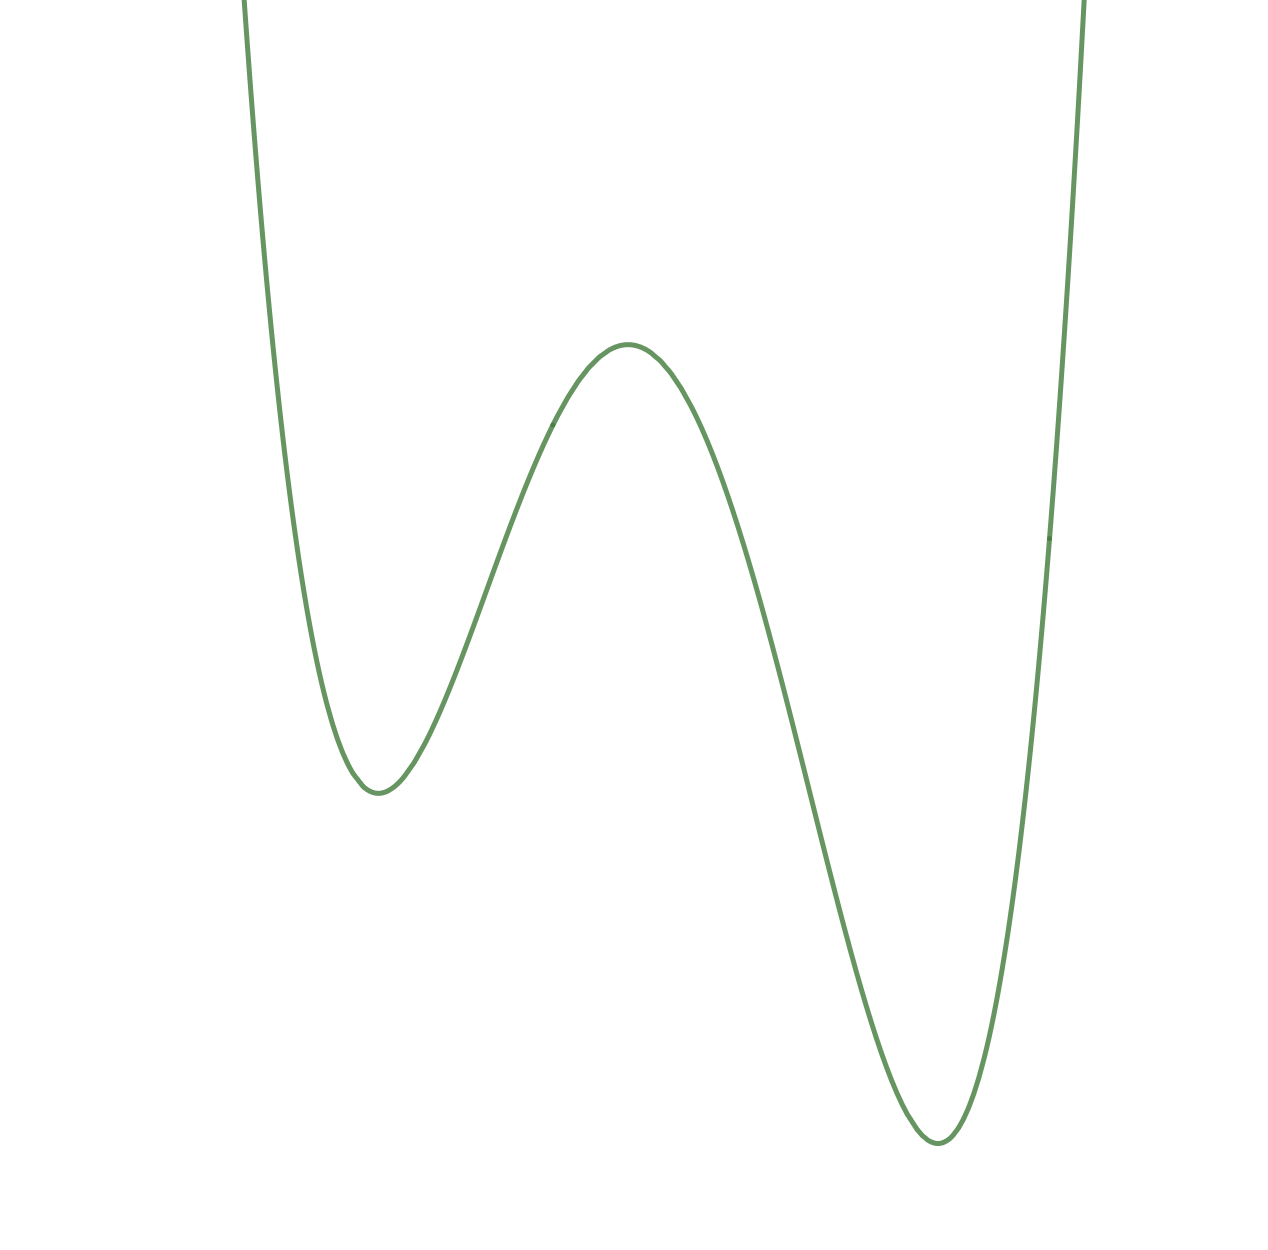
\includegraphics[width=0.3\textwidth]{cartoon}
%\end{figure} 


}

\end{multicols}

\end{enumerate}




\end{document}

